\documentclass[11pt]{article}
% Horizontal Magnetic Dipole over a lossy half-space
\usepackage[utf8]{inputenc} % Use it to include other characters than ABC
\usepackage[cmex10]{amsmath}
\usepackage{mdwmath}
\usepackage{mdwtab}
\usepackage[hidelinks]{hyperref}
% The following is done to hide ugly color boces around the links
\usepackage{xcolor}
\hypersetup{
    colorlinks,
    linkcolor={red!50!black},
    citecolor={blue!50!black},
    urlcolor={blue!80!black}
}
\usepackage{physics} % For using the oridnary derivative nomenclature
\usepackage{datetime} % Insert date and time
\usepackage[letterpaper, margin=1in]{geometry}
\usepackage{graphicx}
\usepackage{pgfplots}
\usepackage{tikz}
\usepackage{standalone}
\usepackage[americanresistors,americaninductors]{circuitikz}
\usetikzlibrary{positioning}
\usetikzlibrary{arrows}
\usepackage{subfig}
\usepackage{mathptmx} % Times new Roman

% ------------------------------- Useful Tricks Learnt
% Use ={}& to align subequations to the left
% Use = for single equations
% Put comments % in between the lines in order to avoid forming a new paragraph.
% To enter special characters into Inkspace figures, use Ctrl+U and then enter       the unicode. e.g., for \times symbol, the unicode is U+0D7. So the key entry would be Ctrl+U U+0d7 and then press enter.
%
% ----------------- To compile with references use the following order in Shell"
% 1. pdflatex filename.tex
% 2. bibtex filename (no extension)
% 3. bibtex filename (no extension)
% 4. pdflatex filename.tex
% -----------------

% Personal definitions
% Operators
\renewcommand{\v}[1]{\mathbf{#1}} % vectors
\newcommand{\ti}[1]{\tilde{#1}} % spectral representation

% Symbols
\renewcommand{\O}{\omega}  % omega
\newcommand{\E}{\varepsilon}  % epsilon
\renewcommand{\u}{\mu}  % mu
\newcommand{\p}{\rho}  % rho
\newcommand{\x}{\times}  % times
\renewcommand{\inf}{\infty}  % infinity
\newcommand{\infint}{\int\limits_{-\inf}^\inf} % integral by R
\newcommand{\del}{\nabla}  % nabla operator
\renewcommand{\^}{\hat}  % unit vector
\newcommand*\diff{\mathop{}\!\mathrm{d}} % Define differential operator

\definecolor{s1}{RGB}{204, 76, 2}

\begin{document}
  \title{\textsc{Numerical Integration of Sommerfeld Integrals}\\}
  \date{\footnote{Last Modified: \currenttime, \today.}}
  \maketitle

  The fields of sources in a layered media environment involves computation of Sommerfeld Integrals which are reminiscent of a Hankel transform (a Fourier transform in cylindrical coordinate system):

  \begin{equation}
    \int_{0}^{\inf} \ti{G}(k_{\p}; \v{r}|\v{r}') J_n(k_{\p} \p) k_{\p} \diff{k_{\p}}
    \label{eq:SI}
  \end{equation}

  where $\ti{G}$ is a spectral domain Green's function of the structure, $\v{r}$ and $\v{r}'$ are the observation and source locations respectively, and $J_n$ is bessel's function of order $n$. In most cases, the integral in (\ref{eq:SI}) cannot be solved analytically. The integrand exhibits branch point singularities and very slow rate of convergence due to oscillaotory behaviour of the bessel function. Therefore, intelligent methods need to be implemented to expediete the integration of such integrals. By invoking the Cauchy's Integral Theoerem, \cite[p. 377]{arfken2001mathematical} we choose the path of integration along the positive real axis in the complex $k_{\p}$ plane as shown in Fig. \ref{fig:path} with slight indentation into the first quadrant around possible singularities.
  \cite{golubovic2012efficient,michalski2016efficient}

  \begin{figure}[h!]
    \centering
    \includestandalone[width=1\textwidth]{figures/path}
    \caption{Integration Path along the real axis}
    \label{fig:path}
  \end{figure}

The integral in (\ref{eq:SI}) is computed by splitting into three sections:

\begin{equation}
  \int_{0}^{\inf} \ti{G}(k_{\p}; \v{r}|\v{r}') J_n(k_{\p} \p) k_{\p} \diff{k_{\p}} = \left(\int_{0}^{\gamma} + \int_{\gamma}^{a} + \int_{a}^{\inf} \right)
  \ti{G}(k_{\p}; \v{r}|\v{r}') J_n(k_{\p} \p) k_{\p} \diff{k_{\p}}
  \label{eq:SI_split}
\end{equation}

where $\gamma$ represents the detour from the real axis. The distance between $\gamma$ and the real axis should be kept small in order to avoid wild growth of the bessel function with increasing imaginary part as illustrated in Fig. \ref{fig:bessel}. The path detour ends at the breakpoint $a$, where the method of numerical integration is switched. The two finite interval integrals in (\ref{eq:SI_split}) are computed using Double Exponential (DE) quadrature rule. \cite{takahasi1974double}. Unlike other quadratures, the DE rule works efficiently on integrands with singularity at one or both of the endpoints. \cite{bailey2005comparison, mori2005discovery} The remaining infinite interval along the real axis is computed through Partition Extrapolation (PE) method

\begin{figure}[h!]
  \centering
  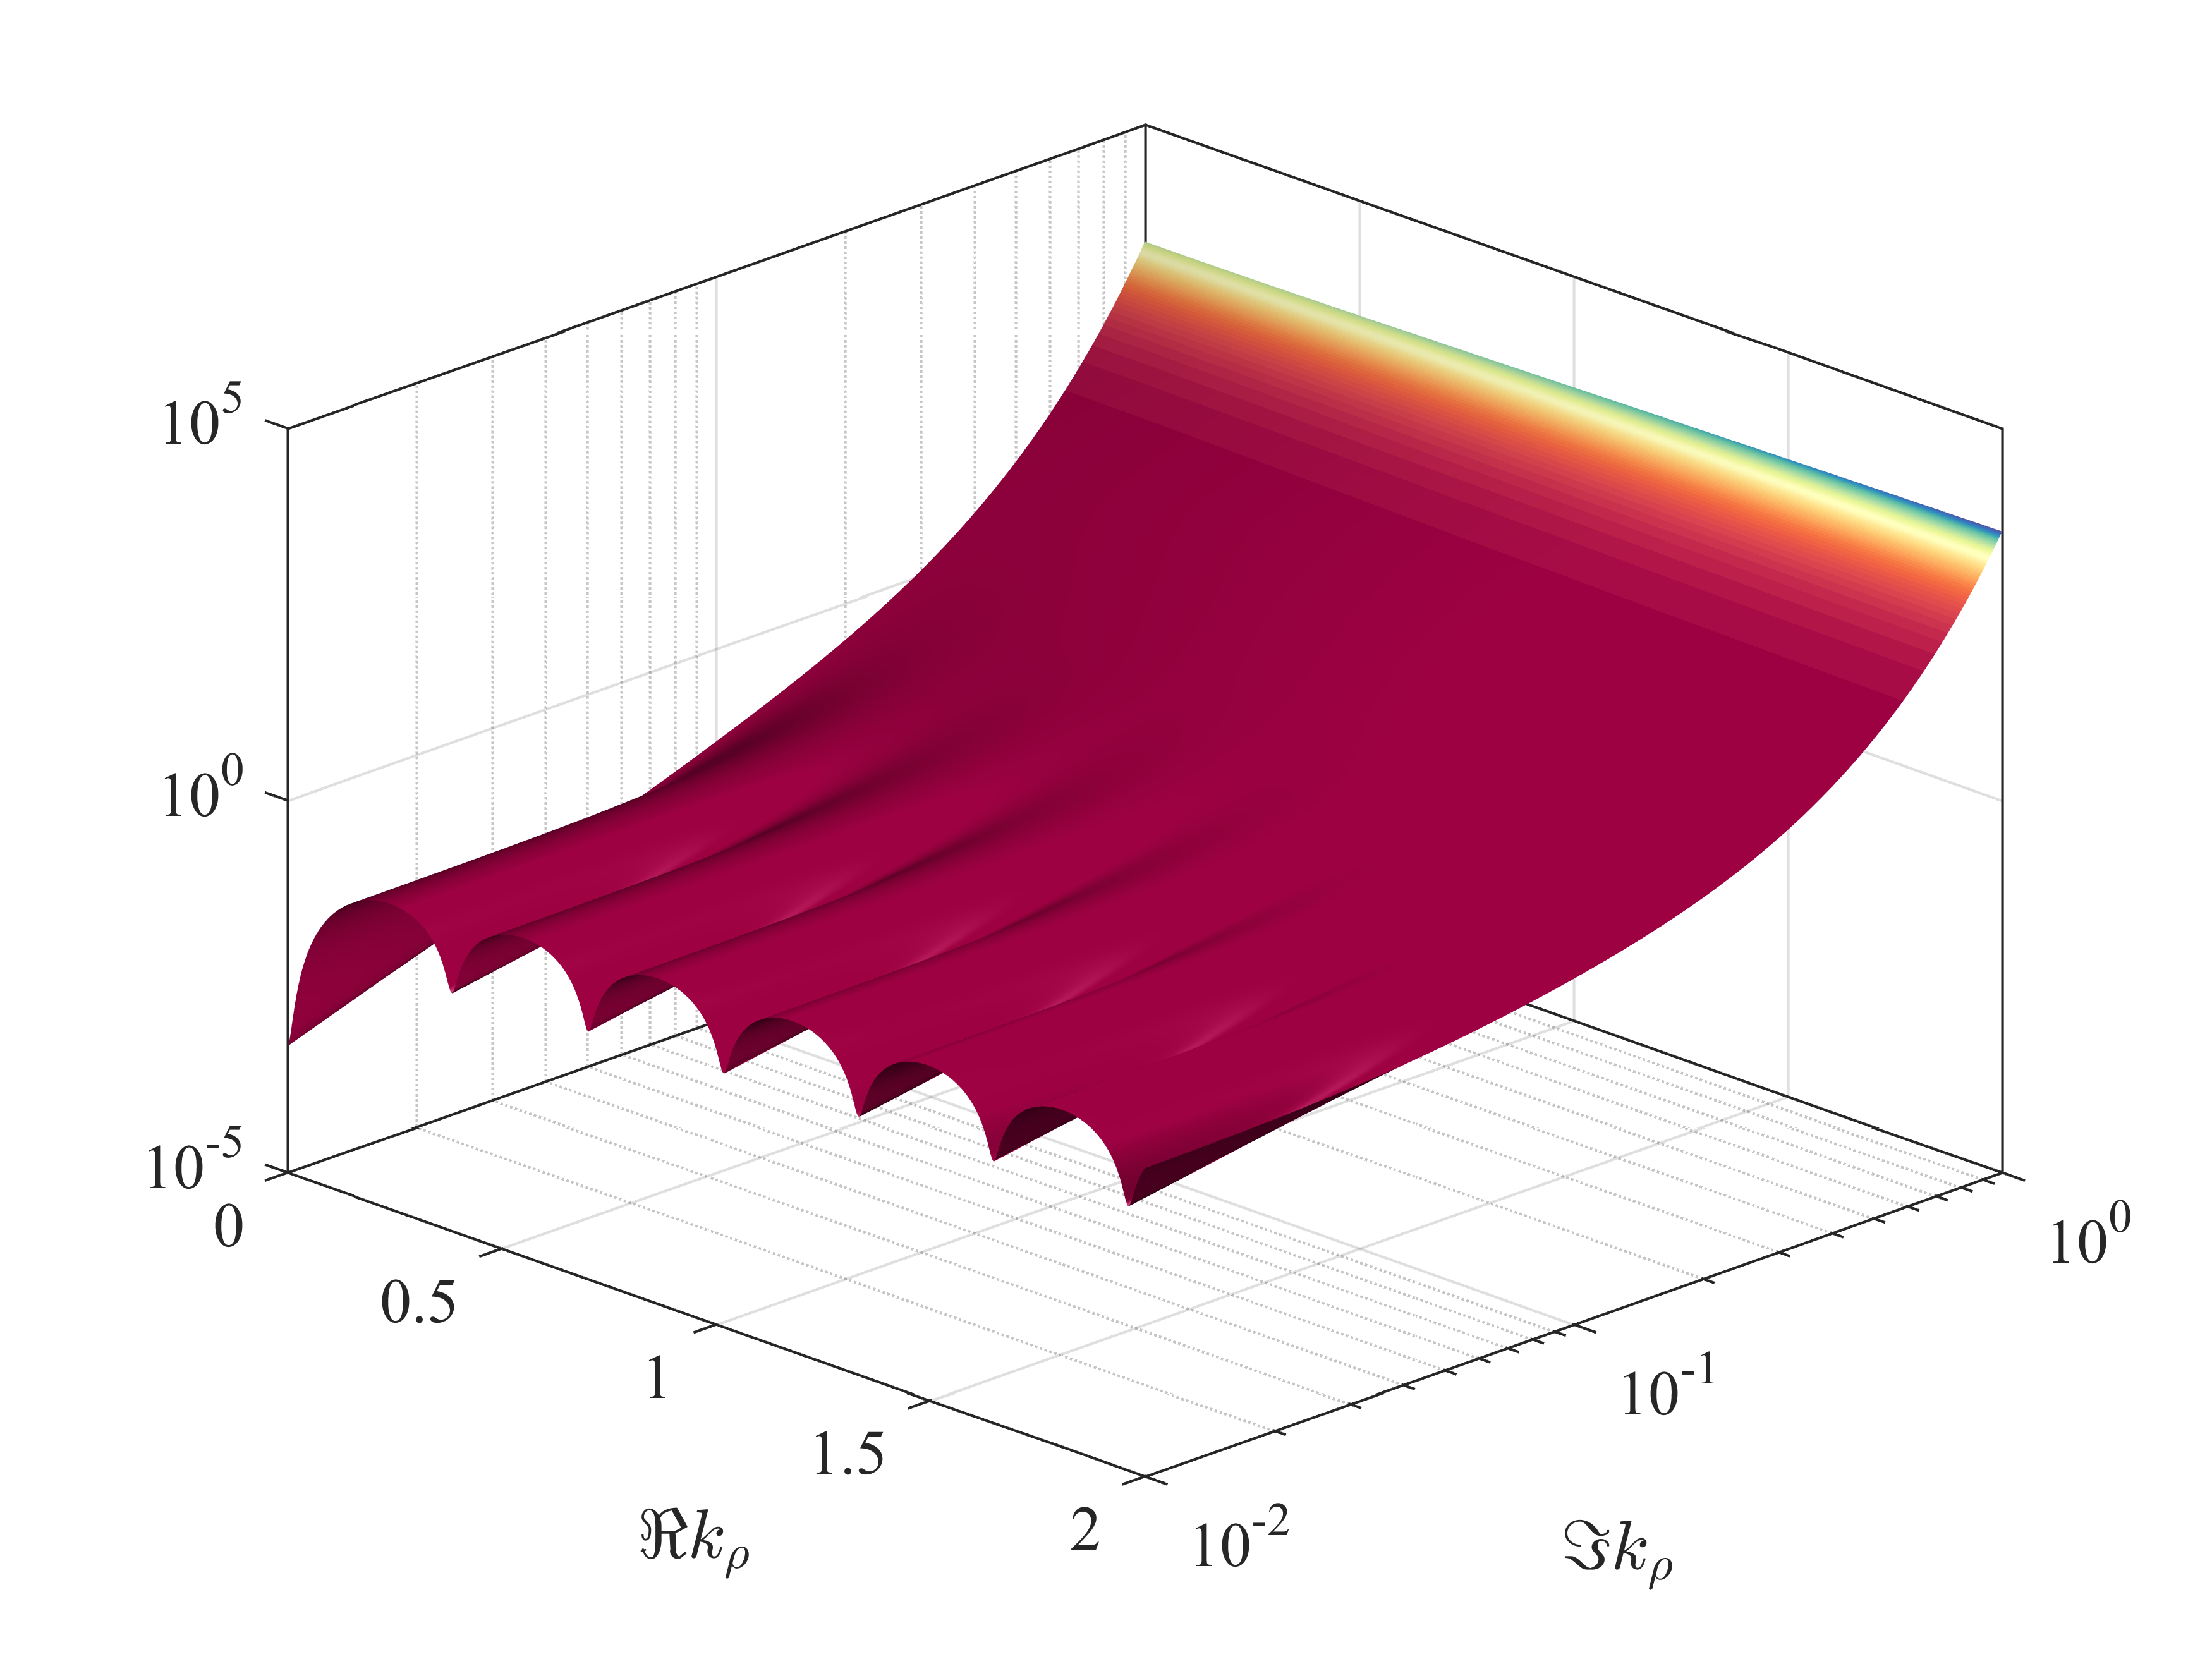
\includegraphics[width=\textwidth]{figures/J_1_comp.png}
  \caption{Exponential Growth of Bessel function $J_1(10 k_{\p})$ along the imaginary axis}
  \label{fig:bessel}
\end{figure}

\section{Overview of Numerical Integration}

Most numerical integration routines are based on polynomial interpolation where the integral is approximated by:

\begin{equation}
  \int_a^b f(x) \diff(x) \approx w_0 f(x_0) + w_1 f(x_1) + ... + w_n f(x_n) = \sum_{i = 0}^n w_i f(x_i)
  \label{eq:Num_int}
\end{equation}

\section{Far Field Computation}

Far-fields due to sources present in a layered media are of interest in many situations. Asymptotic expressions of the fields in the near field have to be derived. According to the Sommerfeld radiation condition \cite[p. 189]{sommerfeld1949partial}, the fields must decay at the rate of $r^{-1}$, and therefore,  asymptotic behaviour of the far-field should follow such. However, fields that propagate along an interface (surface waves) have decay rate of $r^{-1/2}$. Hence, in the presence of layered media, a closed-form expression for the far-fields can not be obtained. \cite[p. 346]{novotny2006principles}[p. 346] If the regions close to the multilayer are excluded, closed-form expressions of the far-field can be derived. \cite[p. 1183]{michalski2005electromagnetic}


  \clearpage % Force Bibliography to the end of document
  \bibliography{refs}
  \bibliographystyle{ieeetr}

\end{document}
